\documentclass[main]{subfiles}

\begin{document}


\chapter{Pruebas sobre el controlador}
\label{chap:test_control}

El objetivo de la presente secci\'on es el de analizar el desempeño del controlador. En primer lugar realizaremos un estudio en lo que respecta a la respuesta al escal\'on para las tres trayectorias definidas en el cap\'itulo \ref{chap:linealizacion}, luego analizaremos como es el comportamiento del sistema frente a medidas con ruido para finalmente estudiar el desempeño del controlador frente a errores y no idealidades en el modelado del sistema.\\

En lo que respecta al an\'alisis de la respuesta del controlador ante la presencia de ruido en las medidas se utilizar\'a la funci\'on del simulador desarrollado que nos permite agregar a cada estado un ruido que cumple con el siguiente modelo:

\begin{equation}
\label{eq:noise}
\eta_i = A_i\cos(\omega t)+\varepsilon(\mu_i,\sigma_i)
\end{equation}

Donde $\varepsilon(\mu_i,\sigma_i)$ es un ruido gaussiano de media $\mu_i$ y de desviaci\'on est\'andar $\sigma_i$.

\section{Respuesta al escal\'on}
Nos centraremos en estudiar las respuestas al escal\'on de los tres tipos de trayectorias. En esta secci\'on no se consideran medidas con ruido, es decir que se conoce el estado a la perfecci\'on.  

\subsection{Trayectoria de hovering}

\subsubsection{Desplazamientos en la direcci\'on vertical}
Se consideran condiciones iniciales nulas. Se fija como setpoint:
\begin{itemize}
\item Prueba 1: ${x_s = 0 m;\quad y_s = 0 m;\quad z_s = 1 m;\quad \theta = 0_s^\circ}$
\item Prueba 2: ${x_s = 0 m;\quad y_s = 0 m;\quad z_s = 7 m;\quad \theta = 0_s^\circ}$
\end{itemize}

No se aprecian variaciones en ninguna de las variables de estado excepto en la posici\'on vertical ($z$) y en la velocidad $v_{q_z}$. La respuesta al escal\'on para las pruebas uno y dos se muestran en la figura \ref{fig:hov_esc_z}. 
\begin{figure}
  \centering
  \subfloat[Escal\'on de altura 1 m]{\label{fig:z_1}
  		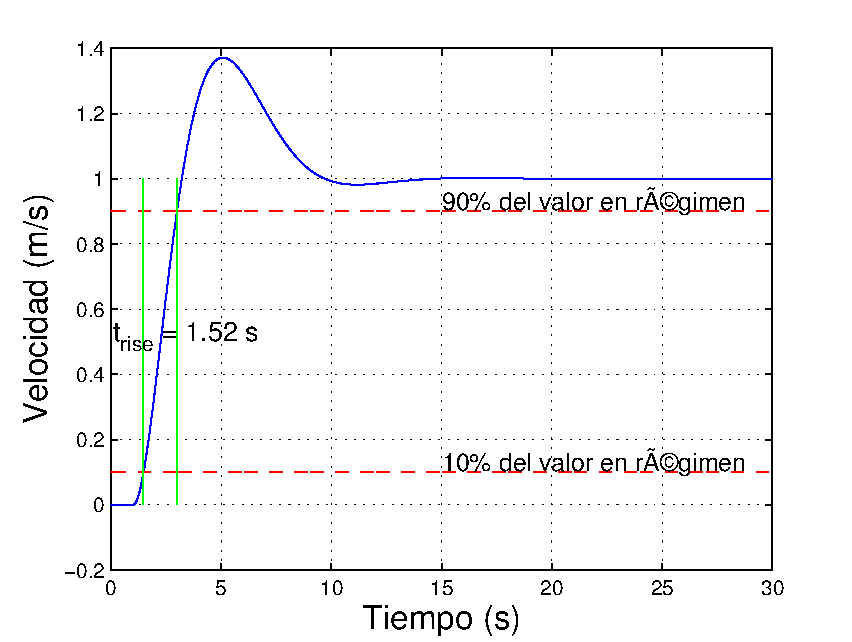
\includegraphics[width=0.5\textwidth]
  			{./pics_test_control/hov/z_1.pdf}}
  \subfloat[Escal\'on de altura 7 m]{\label{fig:z_7}
  		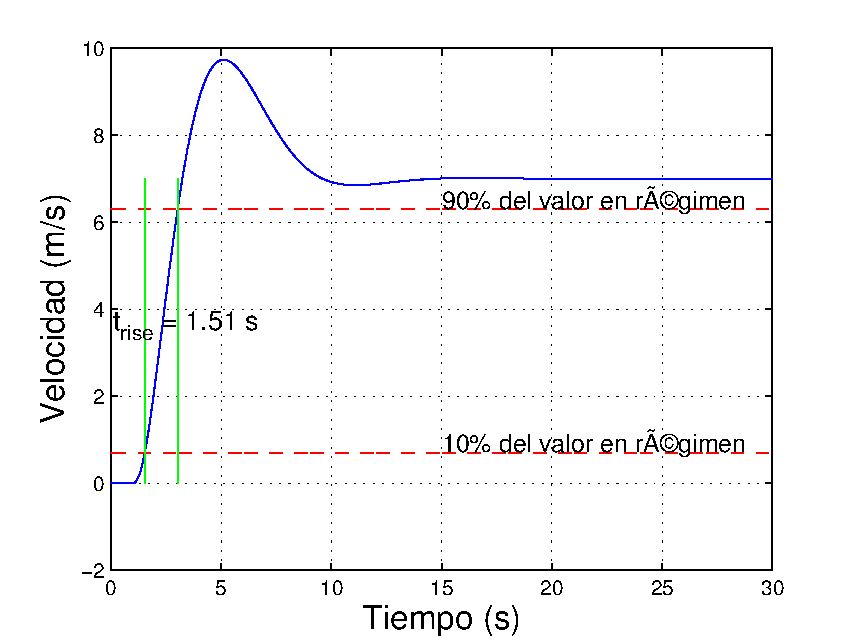
\includegraphics[width=0.5\textwidth]
  			{./pics_test_control/hov/z_7.pdf}}
  \caption{Respuesta al escal\'on en la altura}
  \label{fig:hov_esc_z}
\end{figure}

El tiempo de \emph{rise} de ambas respuestas al escal\'on es considerado ampliamente satisfactorio. El sobretiro obtenido es superior a lo deseable, siendo aproximadamente un $40\%$ del valor en r\'egimen. El mismo puede reducirse otorgando un peso menor en la matriz \ref{eq:Q} a los t\'erminos asociados al estado integrado de la altura. Esta modificaci\'on produce a la vez que el controlador se comporte considerablemente peor frente a variaciones en el sistema. Esto ser\'a analizado con mayor detalle en la secci\'on \ref{sec:robustez}. Existe un compromiso entre los fen\'omenos descriptos, la matriz de realimentaci\'on escogida busca contemplarlos a ambos determinando un valor considerado como \'optimo.\\ 

En la figura \ref{fig:w_z_7} se observa la velocidad angular de uno de los motores para el escal\'on de altura $7m$. Se observa que en los instantes iniciales la velocidad angular de uno de los motores alcanza su valor m\'aximo ($387rad s^{-1}$), por lo tanto no se puede asegurar el perfecto funcionamiento para escalones de mayor altura. Por otra parte se observa en ambas pruebas que una vez alcanzado el valor objetivo se mantiene perfectamente.\\

\begin{figure}
  \centering
	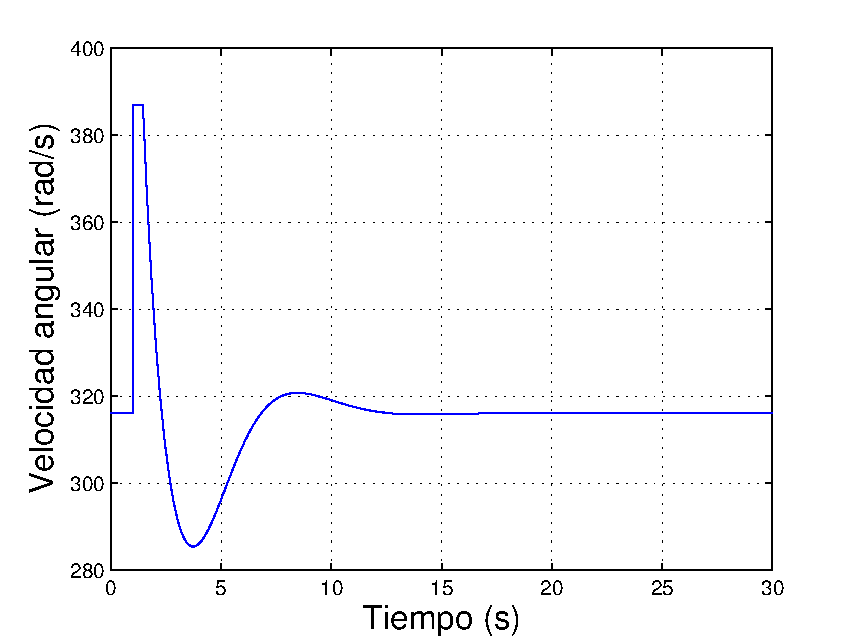
\includegraphics[width=0.5\textwidth]{./pics_test_control/hov/w_z_7.pdf}
  \caption{Velocidad angular del motor 1 durante un escal\'on de altura $7m$}
  \label{fig:w_z_7}
\end{figure}


\subsubsection{Desplazamientos en la direcci\'on horizontal}
Partiendo de condiciones iniciales nulas excepto la altura donde se considera $z = 3 m$, se fija el siguiente setpoint:
\begin{itemize}
\item ${x_s = 5 m;\quad y_s = 0 m;\quad z_s = 3 m;\quad \theta = 0_s^\circ}$
\end{itemize}

En la figura \ref{fig:hov_esc_x} se observan las car\'acteristicas m\'as importantes de la trayectoria. Para lograr un desplazamiento en alguna direcci\'on horizontal el cuadric\'optero debe realizar al menos un giro seg\'un los \'angulos de pitch o roll. Esto se observa claramente en la figura \ref{fig:axis_x_5}. Este giro produce una variaci\'on en la altura. Para el caso considerado, dicha variaci\'on es inferior a los $25cm$, valor que se considera aceptable. Para mayores escalones en la direcci\'on horizontal se observan variaciones de altura no deseables. Por otra parte en lo que respecta a la respuesta al escal\'on en la direcci\'on $\vec{i}_I$ se tiene un tiempo de \emph{rise} y un sobretiro muy similar que en el caso del escal\'on vertical.\\

En resumen, el controlador diseñado se comporta adecuadamente para la condici\'on de hovering, cabe recordar que la linealizaci\'on realizada para dicha trayectoria supone el reposo del sistema y los desplazamientos no se encuentran a priori contemplados en dicha trayectoria. El controlador diseñado nos permite algunos desplazamientos con un buen tiempo de respuesta, para desplazamientos de mayores distancias se debe trabajar o bien con rectas o c\'irculos. 

\begin{figure}
  \centering
  \subfloat[Ejes solidarios al cuadric\'optero a lo largo del tiempo]{\label{fig:axis_x_5}
  		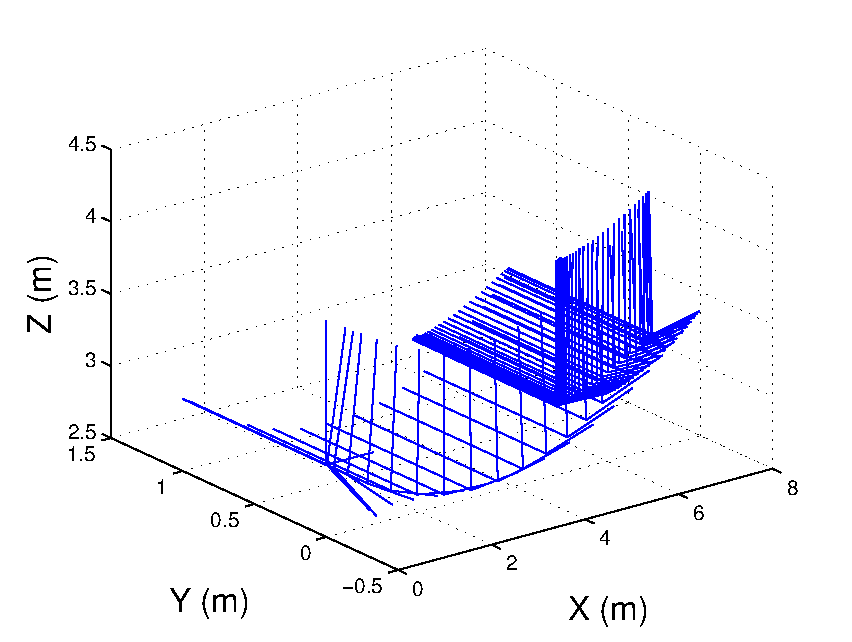
\includegraphics[width=0.35\textwidth]
  			{./pics_test_control/hov/axis_x_5.pdf}}
  \subfloat[Posici\'on seg\'un $\vec{i}_I$]{\label{fig:x_5}
  		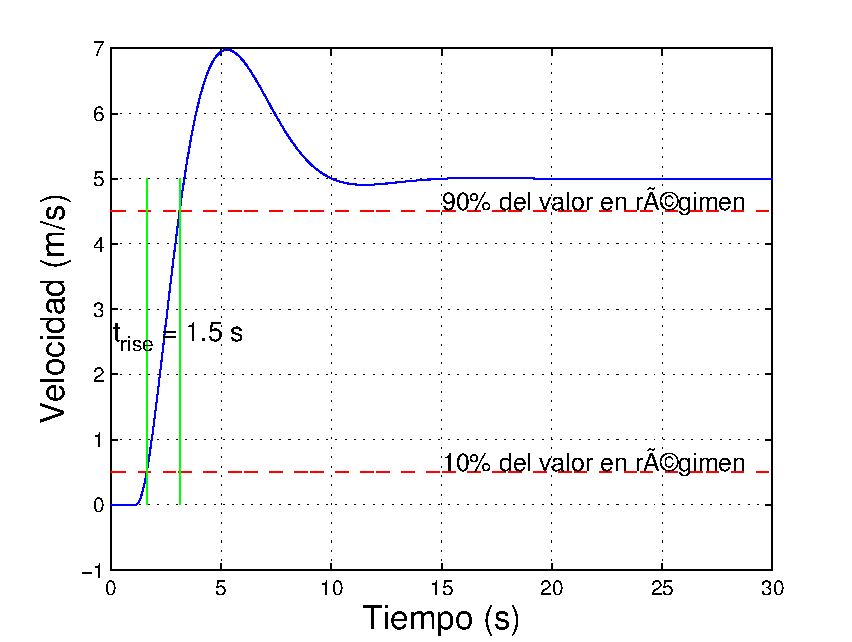
\includegraphics[width=0.35\textwidth]
  			{./pics_test_control/hov/x_5.pdf}}
  \subfloat[Altura en m]{\label{fig:z_x_5}
  		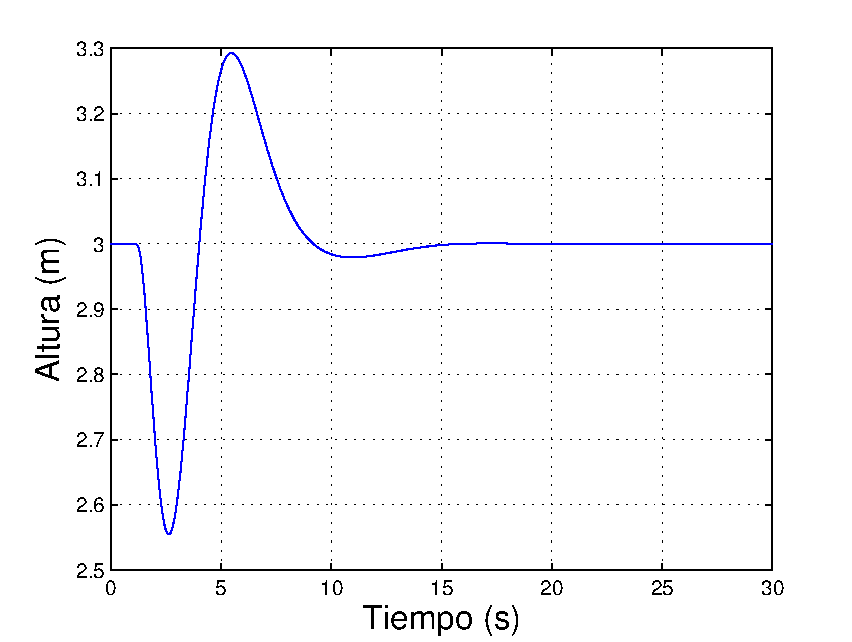
\includegraphics[width=0.35\textwidth]
  			{./pics_test_control/hov/z_x_5.pdf}}
 
  \caption{Escal\'on de 2m en la direcci\'on horizontal}
  \label{fig:hov_esc_x}
\end{figure}

\section{Robustez frente a la presencia de ruido de medici\'on}

Hasta aqu\'i hemos evaluado las caracter\'isticas del controlador diseñado en situaciones en las cuales se conoce exactamente el vector de estados, evidentemente la situaci\'on de vuelo real no se corresponde con esta idealidad. Las medidas realizadas tienen ruido intr\'inseco, muy superior a los considerados en las pruebas de calibraci\'on y caracterizaci\'on de los sensores. El aumento de este ruido se debe principalmente a las vibraciones mec\'anicas que introducen las h\'elices.\\

Resulta fundamental conocer en forma aproximada el comportamiento de los ruidos de medida. Con dicho fin se realiz\'o una prueba de vuelo en la cual el cuadric\'optero estaba sujeto por arriba y por debajo quedando imposibilitado de realizar movimientos. Se comandaron los motores a la velocidad de hovering. En la presente secci\'on se presentan los par\'ametros de la ecuaci\'on \ref{eq:noise} que mejor ajustan el ruido. Si bien se podr\'ia haber realizado dicho ajuste utilizando m\'inimos cuadrados, al menos para la parte del ruido no aleatorio, se opt\'o por realizar dicho ajuste en forma iterativa.\\

Dado que los \'angulos de pitch y de roll se obtienen directamente con los aceler\'ometros los ruidos asociados a ambas medidas son id\'enticas. Por dicho motivo consideraremos un solo ruido replicado en ambas variables. En el caso de las velocidades angulares y de la posici\'on horizontal (medida con el GPS), trabajaremos de la misma forma.\\ 

Finalmente cabe aclarar que se espera que los ruidos obtenidos sean independientes del tipo de trayectoria realizada, por lo tanto los ruidos obtenidos para la trayectoria de hovering ser\'an los utilizados para las restantes. 
\subsection{Hovering}

Para el ruido asociado a las medidas de los \'angulos de pitch y de roll se escogieron los siguientes par\'ametros:

\begin{itemize}
\item $A_{roll} = 0.05^\circ$
\item $\omega_{i_{roll}} = 2\pi 0.03 rads^{-1}$
\item $\sigma_{roll} = 6.05^\circ$
\item $\mu_{roll} = 0.27 ^\circ$
\end{itemize}
  
En la figura \ref{fig:ruido_roll} pueden compararse los ruidos obtendidos en la ``situaci\'on de vuelo'' descripta anteriormente y el ruido en la simulaci\'on. Asimismo puede observarse como, a pesar de la gran presencia de ruido la variable de estado de inter\'es se mantiene controlada muy cercana al valor deseado. El valor m\'aximo y m\'inimo de roll alcanzados son $6.48^\circ$ y $-6.41^\circ$.\\

En la figura \ref{fig:roll_vuelo} se observan tres amplitudes de ruido bien marcadas. La primera corresponde a las medidas con los motores apagados, la segunda a partir del segundo 20.5 donde los motores operan a velocidad m\'inima ($109 rev s^{-1}$) y la tercera a partir del segundo 34 donde la velocidad angular de los motores es igual a la velocidad de hovering. En lo que sigue del an\'alisis nos concentraremos exclusivamente en esta tercer etapa.\\

\begin{figure}
  \centering
  \subfloat[Medida del \'angulo de Roll en ``situaci\'on de vuelo'']{\label{fig:roll_vuelo}
  		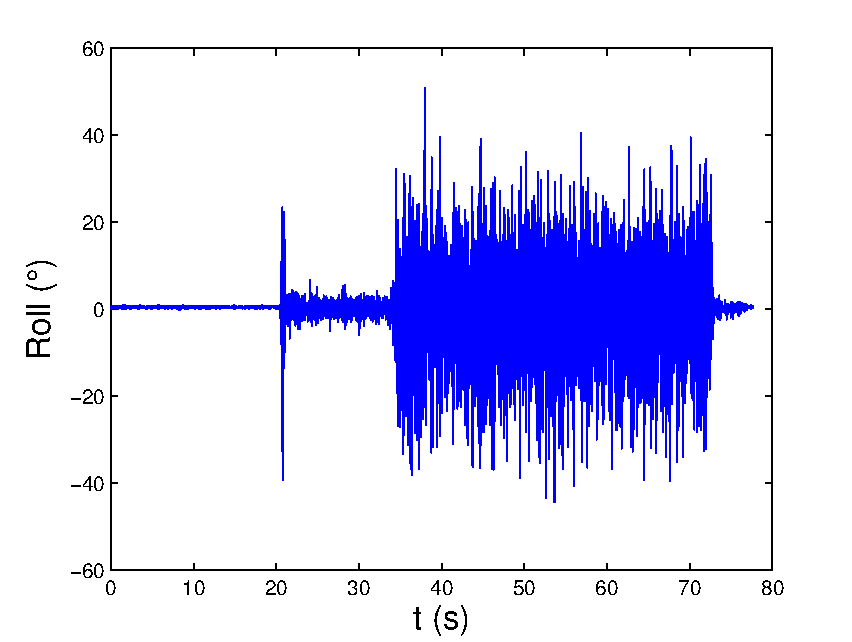
\includegraphics[width=0.5\textwidth]
  			{./pics_test_control/ruido/roll_vuelo.pdf}}
  \subfloat[Ruido de Roll simulado y Roll efectivo ]{\label{fig:roll_noise}
  		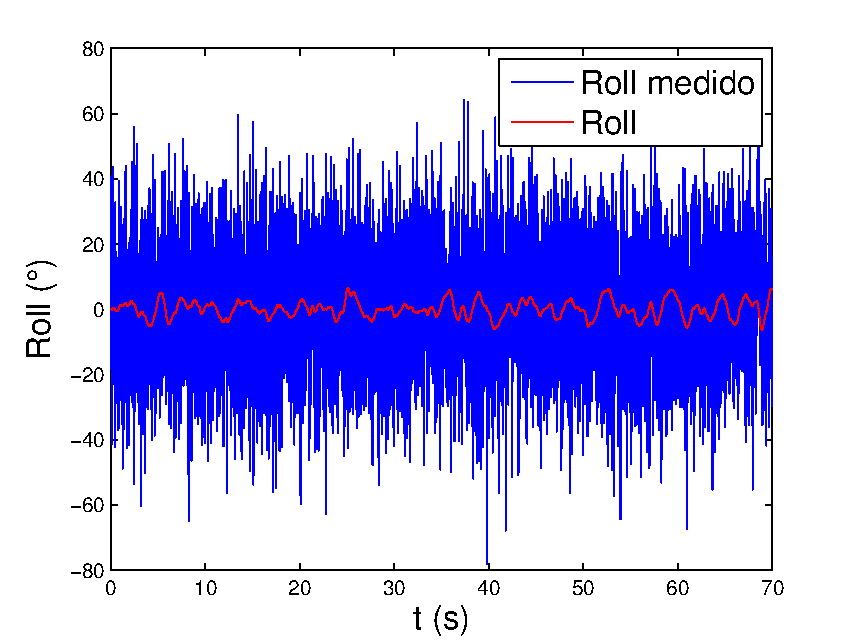
\includegraphics[width=0.5\textwidth]
  			{./pics_test_control/ruido/roll_noise.pdf}}
  \caption{Ruidos de Roll}
  \label{fig:ruidos_roll}
\end{figure}
  
El \'angulo de Yaw se determina adem\'as utilizando la lectura del magnet\'ometro, por dicho motivo se separa el an\'alisis de su ruido de los restantes \'angulos de Euler. En este caso los par\'ametros de ruido utilizados son:

\begin{itemize}
\item $A_{yaw} = 0.23^\circ$
\item $\omega_{yaw} = 2\pi 0.07 rad s^{-1}$
\item $\sigma_{yaw} = 2\circ$
\item $\mu_{yaw} = 0$
\end{itemize}

En la figura \ref{fig:ruidos_yaw} puede observarse como, a pesar del ruido en la medida el controlador se mantiene robusto apart\'ndose del valor objetivo $0.96^\circ$ en el peor de los casos. El resultado en lo que respecta al control de la velocidad angular del sistema es similar. En la figura \ref{fig:ruidos_wqx} pueden observarse las gr\'aficas de los ruidos medido y simulado, adem\'as de la velocidad angular ``real''. Se trabaja en este caso con la velocidad angular $\omega_{q_x}$. Los par\'ametros de ruido escogidos son:
\begin{itemize}
\item $A_{\omega_{q_x}} = 0.03^\circ s^{-1}$
\item $\omega_{\omega_{q_x}} = 2\pi 0.03 rad s^{-1}$
\item $\sigma_{\omega_{q_x}} = 0.64\circ s^{-1}$
\item $\mu_{\omega_{q_x}} = 0$
\end{itemize}
\begin{figure}
  \centering
  \subfloat[Medida del \'angulo de Yaw en ``situaci\'on de vuelo'']{\label{fig:yaw_vuelo}
  		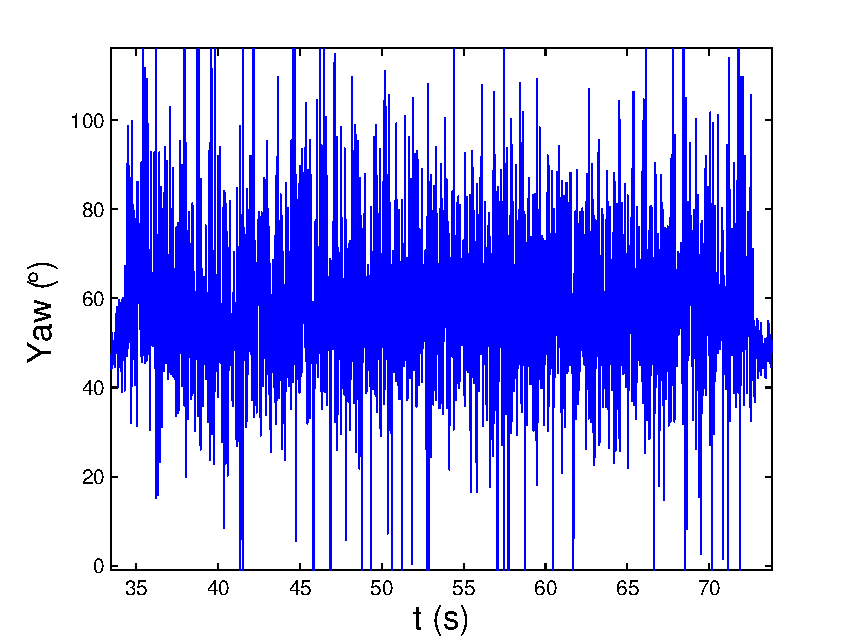
\includegraphics[width=0.5\textwidth]
  			{./pics_test_control/ruido/yaw_vuelo.pdf}}
  \subfloat[Ruido de Yaw simulado y Yaw efectivo ]{\label{fig:yaw_noise}
  		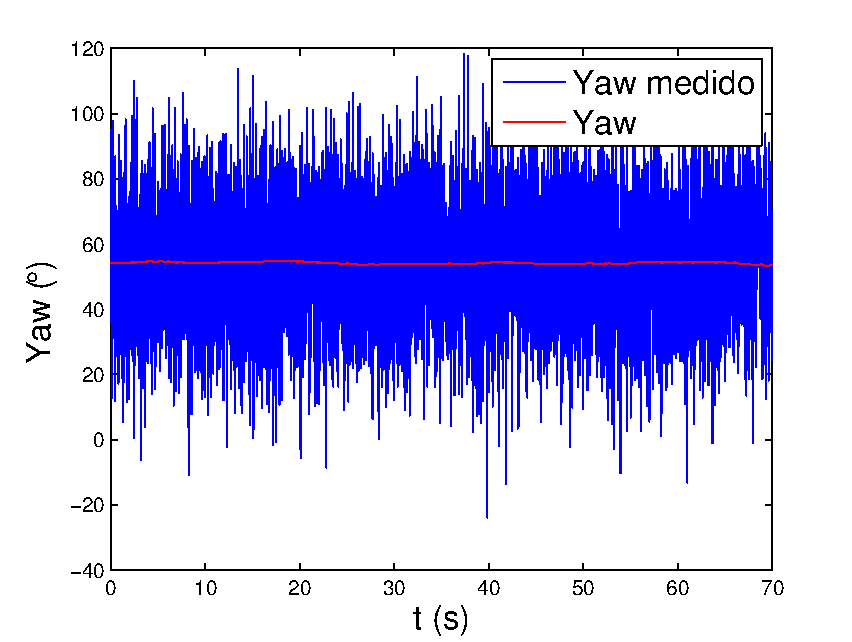
\includegraphics[width=0.5\textwidth]
  			{./pics_test_control/ruido/yaw_noise.pdf}}
  \caption{Ruidos de Yaw}
  \label{fig:ruidos_yaw}
\end{figure}


\begin{figure}
  \centering
  \subfloat[Medida de $\omega_{q_x}$ en ``situaci\'on de vuelo'']{\label{fig:wqx_vuelo}
  		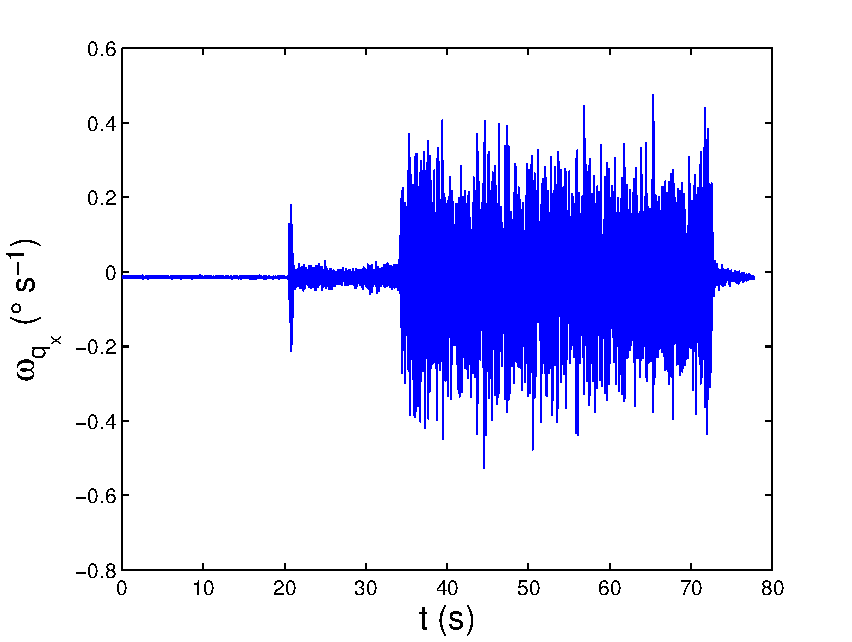
\includegraphics[width=0.5\textwidth]
  			{./pics_test_control/ruido/wqx_vuelo.pdf}}
  \subfloat[Ruido de $\omega_{q_x}$ simulado y $\omega_{q_x}$ efectivo ]{\label{fig:wqx_noise}
  		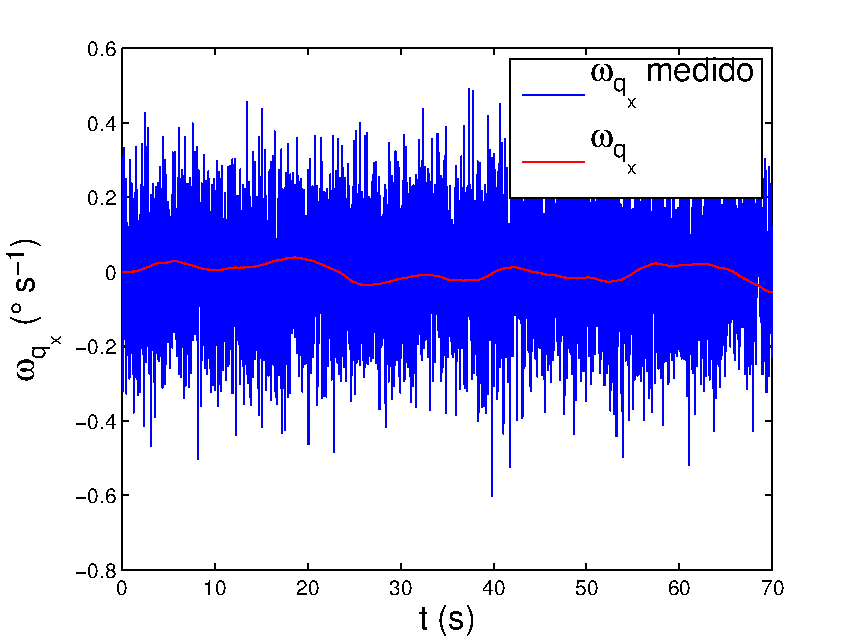
\includegraphics[width=0.5\textwidth]
  			{./pics_test_control/ruido/wqx_noise.pdf}}
  \caption{Ruidos de $\omega_{q_x}$}
  \label{fig:ruidos_wqx}
\end{figure}


Los ruidos observados hasta el momento son preponderamente blancos. Por dicho motivo es practicamente imposible observar la respuesta del control m\'as all\'a de afirmar que efectivamente no nos alejamos sustancialmente de la posici\'on deseada. En el caso del ruido en la altura la situaci\'on es distinta ya que quien juega el papel m\'as importante en el ruido es una oscilaci\'on de baja frecuencia. Los par\'ametros elegidos para representar dicho ruido son:

\begin{itemize}
\item $A_z = 1 m$
\item $\omega_{z} = 2\pi 0.04 rad s^{-1}$
\item $\sigma_{z} = 0.34 m$
\item $\mu_{z} = 0.94 m$
\end{itemize}

\begin{figure}
  \centering
  \subfloat[Medida de z en ``situaci\'on de vuelo'']{\label{fig:z_vuelo}
  		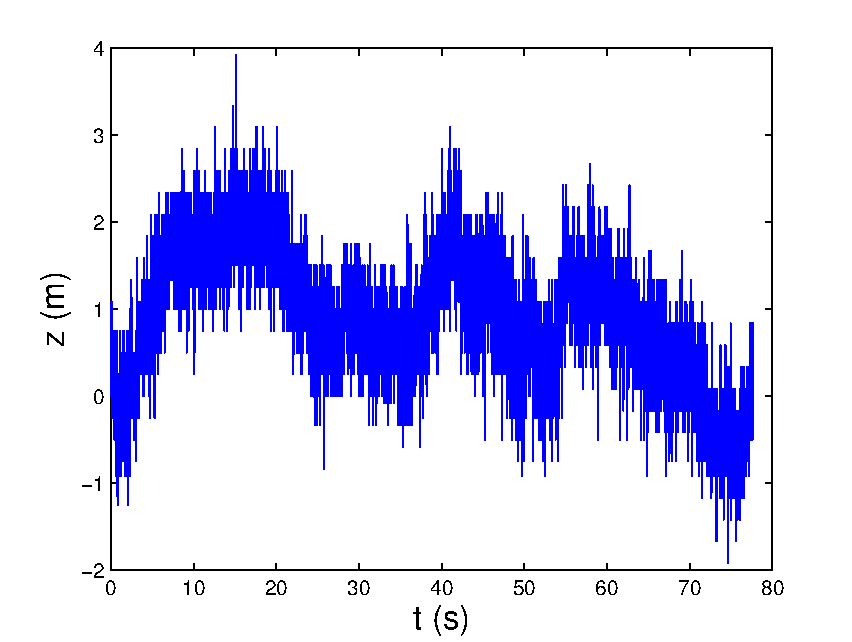
\includegraphics[width=0.5\textwidth]
  			{./pics_test_control/ruido/z_vuelo.pdf}}
  \subfloat[Ruido de z simulado y z efectivo ]{\label{fig:z_noise}
  		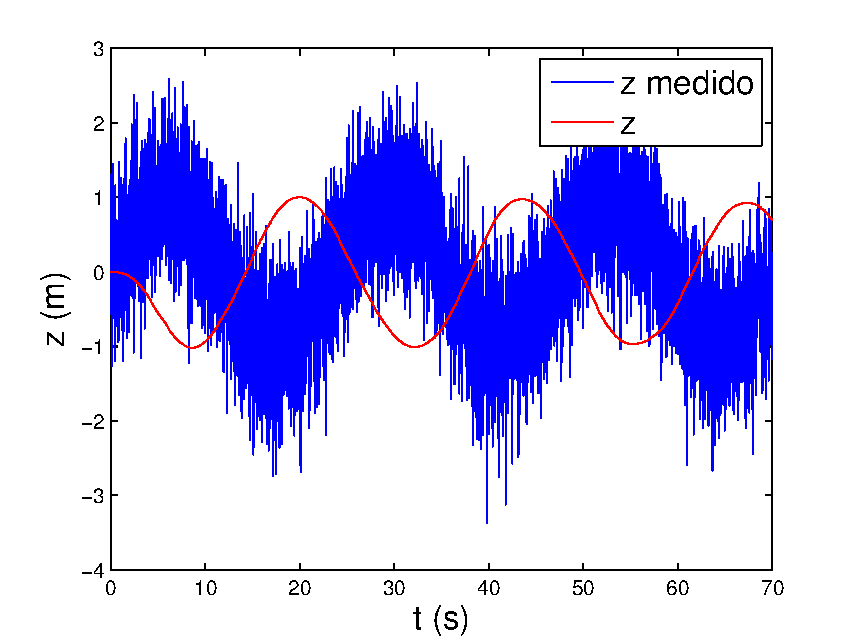
\includegraphics[width=0.5\textwidth]
  			{./pics_test_control/ruido/z_noise.pdf}}
  \caption{Ruidos de z}
  \label{fig:ruidos_z}
\end{figure}

En la figura \ref{fig:z_noise} se aprecia claramente la acci\'on del control ya que para medidas que superan el valor deseado de \emph{setpoint} el control act\'ua en sentido contrario, sucede lo mismo para las medidas que son inferiores al \emph{setpoint}.

Los ruidos que se han menejado hasta aqu\'i corresponden a las medidas directa de los sensores. Al someter estas medidas al filtro de Kalman (ver cap\'itulo \ref{chap:kalman}) tendremos ruidos muy inferiores. Por lo tanto podemos asumir que el sistema se comportar\'a a\'un mejor de lo que se evalu\'o en esta secci\'on.\\

En lo que respecta al ruido de la velocidad no se puede trabajar simplemente con las medidas de los sensores ya que no se tiene ninguna medida directa de la velocidad. La \'unica medida que se tiene es la aceleraci\'on, se podr\'ia integrar dicha medida para obtener valores de velocidad, pero el error introducido en la aceleraci\'on lleva a que la velocidad tenga una deriva, no tiene sentido en pensar esta magnitud con un ruido asociado, excepto que trabajemos en este caso con las estimaciones del vector de estados.\\ 

\section{Robustez frente a variaciones en el modelo}

En este punto nos concentraremos en analizar el comprtamiento del sistema realimentado frente a algunas variaciones en el mismo. Trabajaremos con la trayectoria de hovering, imponiendo como setpoint el reposo y partiendo de esta misma situaci\'on. Analizaremos los dos casos que tienen m\'as importancia pr\'actica: la variaci\'on de la masa y el hecho de que las velocidades angulares de los motores no son id\'enticas.\\ 
\subsection*{Variaci\'on de la masa}
Con condiciones iniciales nulas excepto por la altura que se fija a $3m$, se aumenta la masa del sistema ($1.541kg$) en $200 g$. En la figura \ref{fig:masa} se observa la variaci\'on de la altura por el agregado de masa.


\begin{figure}
  \centering
	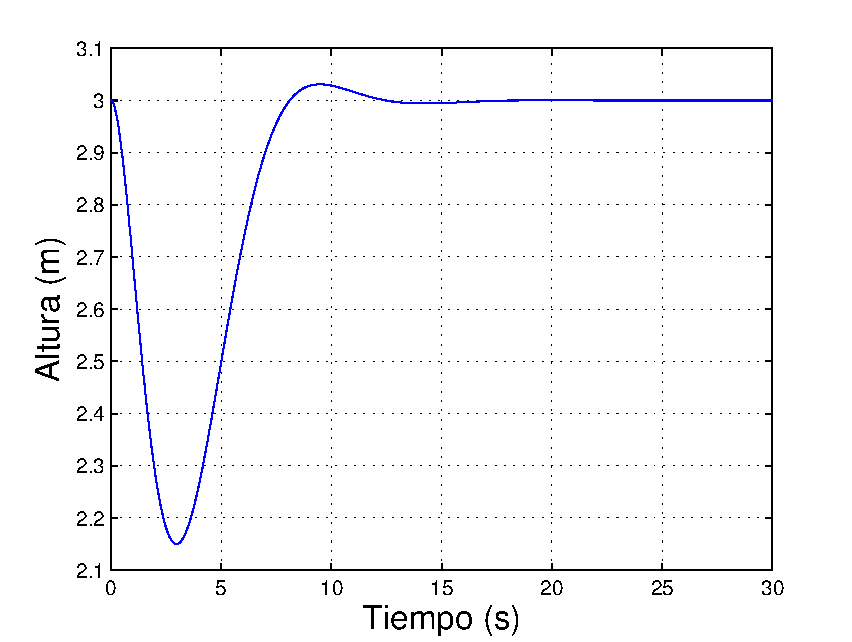
\includegraphics[width=0.5\textwidth]{./pics_test_control/robustez/masa.pdf}
  \caption{Variaci\'on de la altura al agregar una masa adicional de 200g}
  \label{fig:masa}
\end{figure}

La respuesta frente a la variaci\'on de la masa es buena, en menos de diez segundos se vuelve a obtener la altura inicial, adicionalmente la variaci\'on de la altura es inferior a los $90 cm$.  \\

\subsection*{Diferencias entre las velocidades angulares de los motores}

En las mismas condiciones que en la situaci\'on anterior se impone que la velocidad angular del motor 2 cumpla: 
\begin{equation}
\omega_2 = \omega_4 + 15.2rad s^{-1}
\end{equation}

La diferencia de $15.2rads^{-1}$ corresponde a la m\'axima diferencia entre las velocidades angulares de los motores. A priori se espera que esta diferencia produzca un giro positivo en el \'angulo de Roll y un desplazamiento en la direcci\'on $-\vec{j}_I$. Se espera tambi\'en un desplazamiento en la direcci\'on vertical debido a que la fuerza neta es mayor, ya que continuamos asumiendo que $\omega_1 = \omega_2 = \omega_3 =\omega_{hovering}$.\\

En la figura  \ref{fig:motor} se observa la variaci\'on de estas tres variables en funci\'on del tiempo. La inclusi\'on del bloque integrador es fundamental para poder controlar el sistema frente a esta variaci\'on en las velocidades angulares de los motores. Sin dicho bloque el sistema se estabiliza, pero en una posici\'on diferente de la deseada.\\

\begin{figure}
  \centering
  \subfloat[\'Angulo de roll en funci\'on del tiempo]{\label{fig:roll}
  		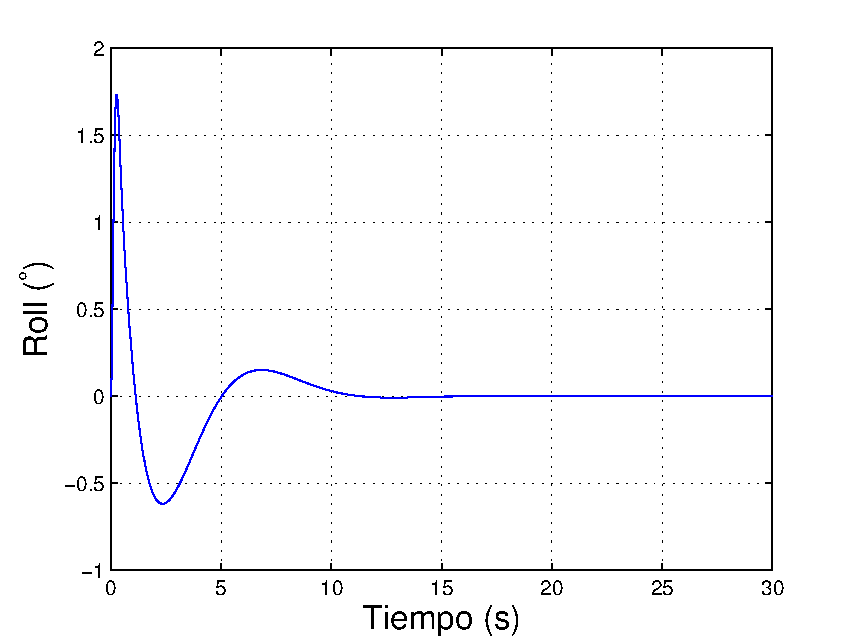
\includegraphics[width=0.35\textwidth]
  			{./pics_test_control/robustez/roll.pdf}}
  \subfloat[Posici\'on seg\'un $\vec{j}_I$]{\label{fig:y}
  		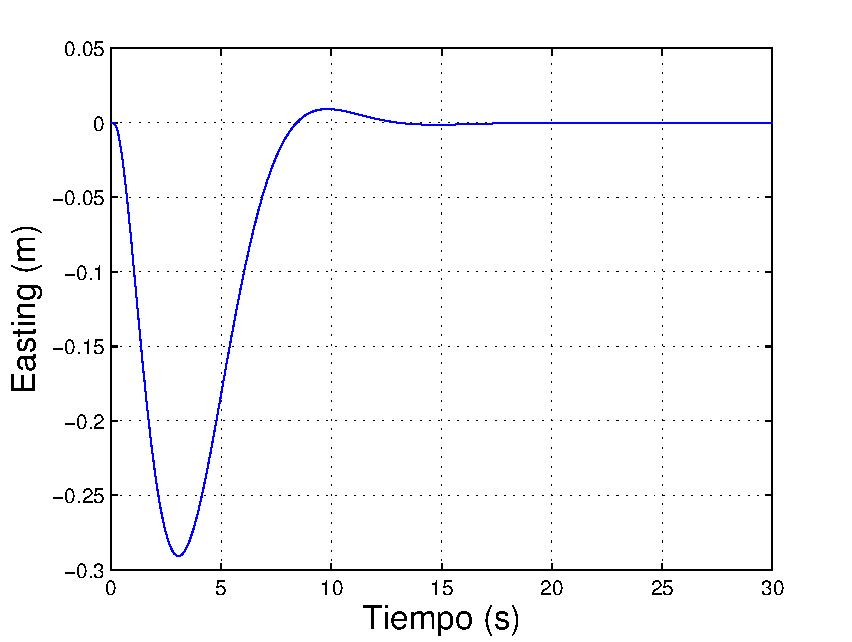
\includegraphics[width=0.35\textwidth]
  			{./pics_test_control/robustez/y.pdf}}
  \subfloat[Altura en m]{\label{fig:z}
  		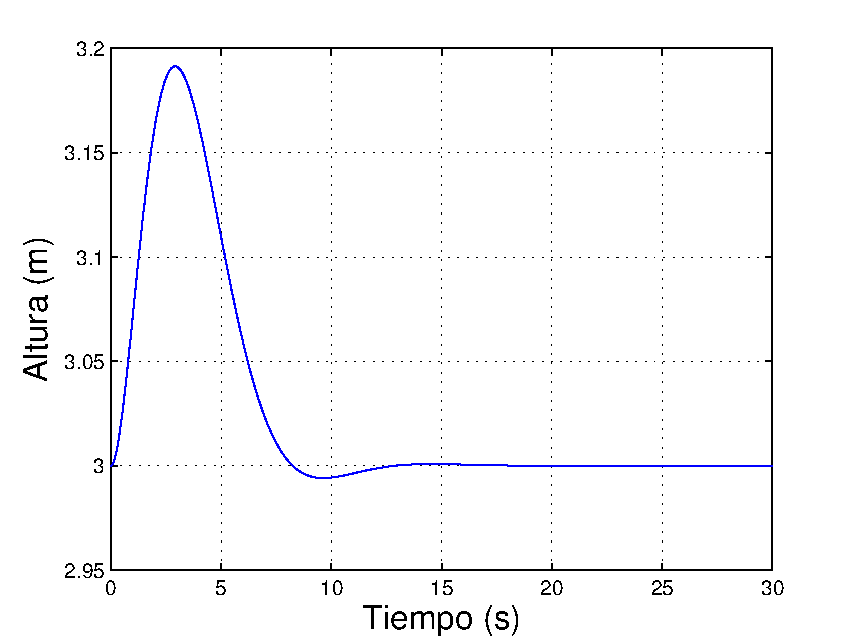
\includegraphics[width=0.35\textwidth]
  			{./pics_test_control/robustez/z.pdf}}
 
  \caption{Diferencia de $15.2 rad s^{-1}$ entre las velocidades angulares de los motores 2 y 4.}
  \label{fig:motor}
\end{figure}


En resumen el controlador diseñado se presenta como satisfactorio ya que permite seguir las trayectorias deseadas con buenos tiempos de respuesta. Por otra parte, su respuesta frente a medidas extremamente ruidosas (en la pr\'actica se trabaja con estados mejor estimados) es muy buena, ya que mantiene al sistema en torno al valor objetivo evidentemente presenta algunas variaciones debidas al error en la medida. Finalmente cabe señalar la robustez del mismo frente a variaciones en el sistema como ser la masa y una diferencia entre las velocidades angulares de los motores.\\

El sobretiro en la respuesta al escal\'on parece superior a lo desead y es un punto que debe mejorarse en el futuro si se desea un control m\'as preciso del sistema. En esta primer aproximaci\'on al problema los sobretiros presentados son aceptables. La mayor dificultad que se encontr\'o al intentar reducir el sobretiro es que el sistema presenta mayores variaciones frente a variaciones de masa o de las velocidades angulares de los motores. Una posibilidad es la de imponer valores mayores en la diagonal de la matriz R definida en \ref{eq:R}. Sin embargo esta soluci\'on implica que el sistema tenga tiempos de respuesta m\'as lentos.\\

La posibilidad de agregar control sobre las derivadas del vector de estados es una linea que no se lleg\'o a investigar debido al tiempo acotado del proyecto. 



\end{document}